El monumento conocido como Ángel de la Independencia (figura \ref{fig:angel_cil}), ubicado en
la Ciudad de México, tiene una altura total de 36 m. Está formado por un prisma
cuadrangular con altura de 2 m y lado de 8 m aproximadamente, le sigue un cubo de 4 m de lado y luego la columna cilíndrica de 2.69 m de diámetro.


\begin{minipage}{0.3\linewidth}
    \begin{figure}[H]
        \centering
        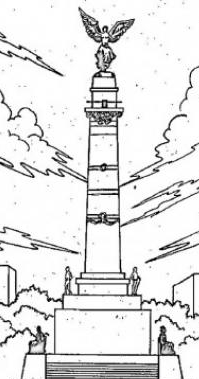
\includegraphics[width=0.8\textwidth]{../images/angel_cil.png}
        \caption{}
        \label{fig:angel_cil}
    \end{figure}
\end{minipage}
\begin{minipage}{0.7\linewidth}
    \begin{parts}
        \part ¿Qué volumen tiene el prisma cuadrangular de la base?

        \begin{solutionbox}{1.5cm}
            128 m$^3$
        \end{solutionbox}

        \part El cubo de la base, ¿qué volumen tiene?

        \begin{solutionbox}{1.5cm}
            64 m$^3$
        \end{solutionbox}

        \part ¿Qué volumen tiene la columna?

        \begin{solutionbox}{2cm}
            La columna es un cilindro de 30 m de altura, por lo que
            \[ V = 170.5 \text{ m}^3 \]
        \end{solutionbox}

        \part ¿Cuál es el volumen total del monumento?

        \begin{solutionbox}{1.5cm}
            $ 128 \text{ m}^3+ 64 \text{ m}^3 + 170.5 \text{ m} = 362.5 \text{ m}^3 $
        \end{solutionbox}
    \end{parts}
\end{minipage}
